% !TEX root = mythesis.tex

%==============================================================================
\chapter{Neutrino Analysis $60^\circ < \theta < 75^\circ$}
\label{sec:tracking}
%==============================================================================
This chapter gives a brief summary of the hardware and the software used to implement tracking for NA64. It begins with a description of the detectors used to track the incoming beam at NA64. Further it describes the algorithm implemented to fit tracks to the information received from the detectors. It ends with a brief description of the software where the said algorithm is implemented.

\section{Detectors}
NA64 uses two varieties of Micro-Pattern Gas Detectors (MPGD) to track the beam particles and estimate their momentum. MPGDs offer a high rate capability along with a spatial resolution O($\mathrm{\mu m}$), both of which are required for NA64. They work on the basic principle that charged particles moving through a medium interact with it in different ways losing some energy in the process. The interaction in case of MPGDs is a direct Coulomb interaction with the atoms present in the detector medium leading to their ionization. The two varieties are the following:
\subsection{MicroMegas}
\label{sec:MM}
MICRO-MEsh GAseous Structure (Micromegas) were invented in 1992 by Georges Charpak and Ioannis Giomataris~\cite{CHARPAK200226} as an alternative to Multi-Wire Proportional Chamber (MWPC)~\cite{Sauli:1977mt} to counter its space resolution and rate limitations.

In a MicroMegas (MM) detector a metallic mesh is introduced between the anode and cathode. The mesh itself is supplied with a high voltage effectively separating the detector volume into two regions. When a charge particle traverses the detector region above the mesh it will ionize the atoms present in the medium. The electrons produced in this process drift towards the mesh where they encounter a high electric field reaching enough energy to create an avalanche. The electrons from the avalanche induce a signal on the readout electrodes while the ions are collected by the mesh. A schematic of the detector is shown in fig.(\ref{fig:Micromegas_na64}) and a more detailed description of the process can be found in \cite{CHARPAK200226}.

The NA64 Micromegas are resistive Micromegas where the usual single readout layer is replaced with a layer of resistive strips (R) followed by additional readout layers below. They were developed at the CERN EP-DT-EF workshop~\cite{Banerjee:2017mdu}. The readout is made up of two layers of 320 strips(X and Y) perpendicular to each other, both rotated by an angle of $45^{\circ}$ with respect to the global reference system and are therefore called U and V throughout the thesis. The strips which are parallel to the resistive strips have a lower capacitive coupling compared to the ones which are perpendicular leading to a slightly worse positional resolution in one plane. The detector was measured to have a gain of $\approx 2 \times  10^4 $ at an amplification voltage of 540 V~\cite{Banerjee:2017mdu}.

\begin{figure}[t!]
\centering
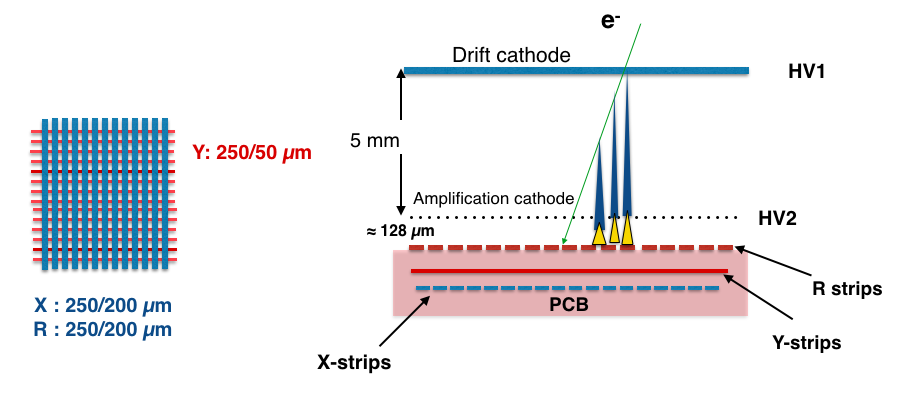
\includegraphics[width=\textwidth]{thesis_figures/NA64_MM.png}
\caption{Left: Strip dimensions of the modules, Right:NA64 Micromega's working principle~\cite{Banerjee:2017mdu}}
\label{fig:Micromegas_na64}
\end{figure}

\subsection{Gas Electron Multiplier}
\label{sec:GEM}
 Gas Electron Multiplier (GEM) was invented by F.Sauli at CERN in 1997. They are cheaper and easier to manufacture compared to other tracking detectors and offer a flexible geometry thus can be used in different shapes and sizes. They have versatile applications as they can be used both as a standalone detector and as readout elements of a Time Projection Chamber (TPC).

 A standard GEM detector consists of a single or multiple layers of  GEM foils inserted between drift and charge collection electrodes. Each foil is made up of polymer coated with a thin metal layer on both sides. The foil is punched with a high density of holes. The holes are etched on both sides of the foil forming a double-conical structure as shown in fig.(\ref{fig:GEM_field}), other kind of hole shapes are also possible. When a differential voltage is applied to the electrodes the holes develop field lines as shown. Electrons drifting through the holes will follow the field lines gaining enough energy to ionize the filled gas leading to an avalanche. Electrons from the avalanche are then collected by the readout  electrode. A more detailed description of the process can be found in~\cite{SAULI20162}.

 The NA64 GEMs were developed at the Technical University Munich (TUM)~\cite{Baust:2008} and resemble the ones developed for COMPASS~\cite{Ketzer:2001dt}. They consist of three stacked GEM foils followed by a stripped readout. The readout consists of two layers perpendicular to each other (X and Y) which are aligned the same as the global reference system. The detector is filled with a mixture of $\mathrm{Ar/CO_2}$ in a ratio of 70/30. The gain of the detector was measured to be $\approx 8 \times 10^4 $ at detector voltage of 4050V~\cite{hosgen:2017}.

 \begin{figure}[t!]
 \centering
   \begin{minipage}[t]{.45\textwidth}
     \centering
     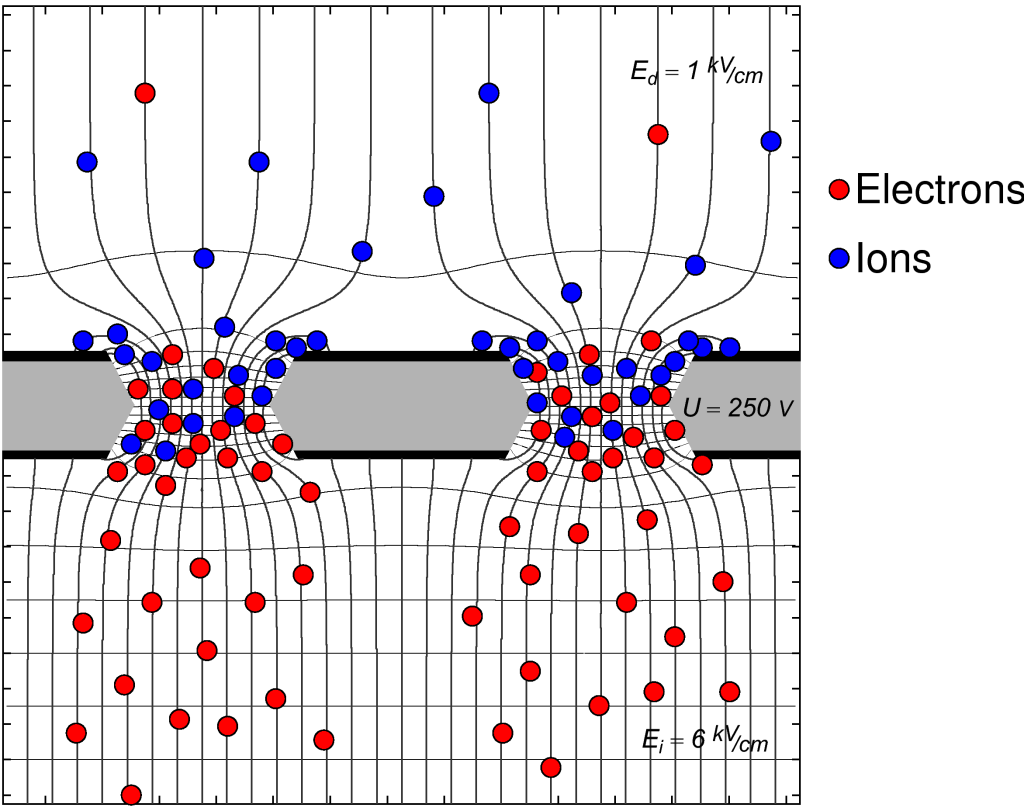
\includegraphics[width=\linewidth]{thesis_figures/GEM_field.png}

     \caption{A sketch of GEM field lines~\cite{GEM_field}.}
     \label{fig:GEM_field}
   \end{minipage}
   \hfill
   \begin{minipage}[t]{.45\textwidth}
     \centering
     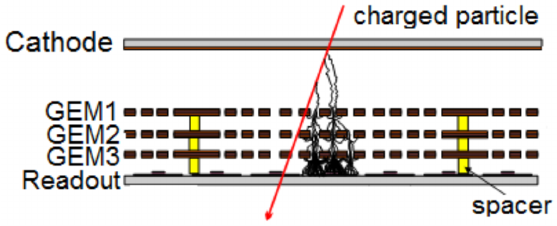
\includegraphics[width=\linewidth]{thesis_figures/GEM_process.png}
     \caption{Schematic of a triple GEM detector along with the working principle~\cite{article_GEM_pic}}
     \label{fig:Triple_GEM}
   \end{minipage}
 \end{figure}

\section{Track-Reconstruction Algorithm}
This section describes the methods used to fit a track to the output obtained from the tracking detectors and to extract momentum information of the beam from this data. For a simple setup this can be done by fitting a straight line through the hits on the detectors for the regions before and after the magnet obtaining the angle between the two lines to estimate the momentum. This method is described under Linear Regression. For a more complex tracking system and to simulate a more realistic picture for the beam and better alignment for the detectors, the Kalman filter algorithm is used to fit the tracks.

\subsection{Linear Regression}
\label{sec:Linear_Regression}
Linear regression for track fitting involves fitting a straight line to the data points, hits in our case with the condition that the total error is minimized. The total uncertainty is calculated as a sum of squares of individual measurement errors. Since the final result is dependent on minimizing the sum of the squares this approach to linear regression is known as least-squares approach. A simple mathematical description of the method is given below.

The equation of a straight line is given by $y=mx + c$, where $m$ is the slope of the line and $c$ is the intercept on the $y$ axis in a Cartesian coordinate system. The final goal is to obtain a good estimate for the two parameters $m$ and $c$. To obtain this estimate the square of error needs to be minimized. The error is the difference between the actual measurement $(x_i,y_i)$ and the prediction from our model, the equation of straight line. This error is also known as the residual and is defined as $r_i = y_i - m x_i - c $ for an $i^{th}$ measurement. Suppose that $n$ hits are measured then to obtain an estimate for $m$ and $c$ we need to minimize $\sum_{i=1}^n r_i^2$. The minimized estimates have the following values:
\begin{equation}
      \text{min}(m) = \frac{\sum_{i=1}^n x_i y-i - 1/n \sum_{i=1}^n x_i \sum_{i=1}^n y-i}{\sum_{i=1}^n x_i^2 - 1/n ()\sum_{i=1}^n x_i)^2}  = \frac{\bar{xy} - \bar{x}\bar{y}}{\bar{x^2-\bar{x}^2}}
\end{equation}
\begin{equation}
      \text{min}(c) = \bar{y} - \text{min}(m) \bar{x}
\end{equation}

A more detailed mathematical description can be found in \cite{Linear_regression}. The quality of the fit can be evaluated by calculating the reduced chi-square $\chi^2_{red}=\frac{\chi^2}{ndf.}=\frac{1}{ndf.}\sum_i \frac{(r_i)^2}{\sigma^2}$ where $\sigma$ is the resolution of each detector which might not be equal and ndf. are the number of degrees of freedom available for the fit.

Linear regression can also be used for NA64 to fit for the bending due to the magnets by replacing the model function from the equation of the straight line to some polynomial function. Such a method is called polynomial regression~\cite{STIGLER1974431}.

\begin{figure}[t!]
\centering
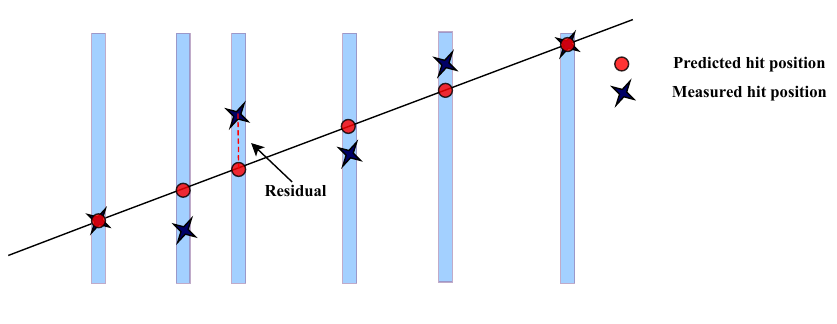
\includegraphics[width=\textwidth]{thesis_figures/linear_reg_new.png}
\caption{Linear regression pictorially. }
\label{fig:linear_regression}
\end{figure}

\subsection{Kalman Filter}
Kalman filter is an estimation technique originally developed to predict rocket trajectories. In particle-physics it is often used as an iterative least-square estimation procedure for track fitting. Following is a brief description of the algorithm for track fitting which closely follows~\cite{Fruhwirth:1987fm,Astier:412374}.

Let's assume for a given track model $x_k$ be the value of the "ideal measurement" at the intersection point between the track and the detector at some point k. This is also called the state vector of the system and in an iterative procedure where the value at location $k$ is obtained from a previous location $k-1$ can be written as :
\begin{equation}
  x_k = f_k(x_{k-1}) + w_k
\end{equation}
where \textbf{f} is the track model propagator function and in this form propogates from detector $k-1$ to $k$ and $w_k$ is a random vector representing the noise between the two detector positions such as multiple scattering perhaps.

\begin{figure}[t!]
\centering
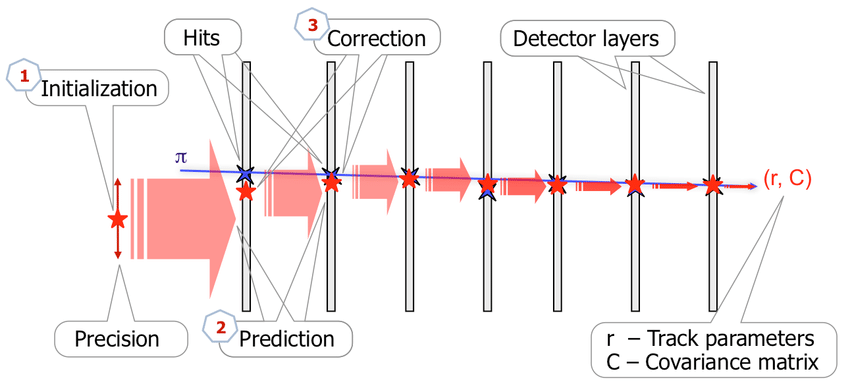
\includegraphics[width=\textwidth]{thesis_figures/KALMAN.png}
\caption{Pictorial representation of the working principle of a Kalman filter ~\cite{article_KALMAN}.}
\label{fig:Kalman_filter}
\end{figure}

Now, the state vector is not a quantity that is measured directly by the detector. If we assume that $m_k$ is the value of the measurement by detector k then it can be given as :
\begin{equation}
  m_k = h_k(x_k) + \epsilon_k
\end{equation}
$h_k(x_k)$ is the function of the state vector measured at the detector which in our case will be a position measurement by our tracking detector. $\epsilon_k$ represents a measurement noise which for an ideal measurement will be zero. We assume that both $w_k$ and $\epsilon_k$ are independent random variables and have a mean value of zero.
For a linearized system,
\begin{equation}
  f_k(x_{k-1}) = F_k x_{k-1}
\end{equation}
\begin{equation}
  h_k(x_{k-1}) = H_k x_k
\end{equation}
There are three key operations that need to be performed for the Kalman filter procedure. These are ordered and described with respect to time specifically to handle multiple scattering in a proper manner.
\begin{description}
  \item $\bullet$~\textbf{Filtering} is estimating the "present" state vector taking into account all the present and "past" measurements. Filtering from $m_1$ to $m_k$ includes filtering $m_1$ to $m_{k-1}$, then propagating from $m_{k-1}$ to $m_k$ and including $m_k$.
  \item $\bullet$~\textbf{Prediction} is estimating the state vector at a "future" time.
  \item $\bullet$~\textbf{Smoothing} is estimating the state vector at any point based on all the measurements.
\end{description}

The basic process can be described as follows. If we have an estimate at position $x_{k-1}$ then it can be extrapolated to position $x_k$ by using the system equation. The estimate at $x_k$ is calculated as a weighted mean between the prediction from the system equation and the measurement from the measurement equation $m_k$. This estimate is passed to all the previous estimates in parallel by using the smoother which is running in a backward direction. Also if there is no process noise $w_k$ then smoothing is equivalent to back extrapolation.

\textbf{System equation:}
\begin{equation}
  x_k = F_k x_{k-1} + w_{k}
\end{equation}
\begin{equation}
  E{w_k} = 0,  \mathrm{Cov[w_k]} = Q_k (1\leq k \leq N)
\end{equation}
\textbf{Measurement Equation:}
\begin{equation}
  m_k = H_k x_{k} + \epsilon_{k}
\end{equation}
\begin{equation}
  E{\epsilon_k} = 0,  \mathrm{Cov[\epsilon_k]} = V_k = G_k^{-1} (1\leq k \leq N)
\end{equation}

As an example here are the different processes for one update step:

\begin{description}
\item $-$ Prediction - Extrapolation of the state vector
      \begin{equation}
        x_k^{k-1} = F_k x_{k-1}
      \end{equation}
      Extrapolation of covariance matrix :
      \begin{equation}
        C_k^{k-1} = F_k C_{k-1} F_k^T + Q_k
      \end{equation}

\item $-$ Filtering - Update of state vector
       \begin{equation}
         x_k = C_k [ \, (C^{k-1}_k)^{-1} x_k^{k-1} + H_k^T G_k m_k ] \,
       \end{equation}
       Update of covariance matrix :
       \begin{equation}
         C_k = [ \, (C^{k-1}_k)^{-1} + H_k^T G_k H_k ]^{-1} \,
       \end{equation}

\item $-$ Smoothing - Smoothed state vector
      \begin{equation}
        x_k^{N} = x_k + A_k(x_{k+1}^N - x_{k+1}^k)
      \end{equation}
      where $A_k$ is called the smoother gain matrix given by: $A_k = C_k F_{k+1} ^T (C_{k+1}^k)^{-1}$

\end{description}
Other information such as residuals $r_k$, covariance matrix of residuals $R_k$ and $\chi^2$ for each step are also calculated and incorporated during the fitting process. A global $\chi^2_{trk}$ is a sum of all chi-squares from filtering. After the Kalman fitting we have three fits for the parameters at a particular hit at position $k$: a track fit for the part upstream i.e  using measurements from 1 till $k$, a backward track fit for the part downstream using measurements from $N$ till $k$ and a fit for the whole track.

The Kalman filter can also be applied for a non-linear system such as in the presence of a magnetic field, by the replacement of the track propagator $f_k$ with the first two terms of of its Taylor series expansion. With this change the procedure is known as extended Kalman filter. This procedure is implemented in the track fitting libraries in CORAL. The computational time of the filter is directly proportional to the number of detector and does not depend much on the total amount of hits in an individual detector. A potential drawback of the algorithm is that it needs initial starting parameters for the state vector and its covariance matrix. This is usually solved by either fitting a small number of measurements with linear regression and then feeding it to the algorithm or by starting with an arbitrary value for the state vector and covariance matrix.

\section{CORAL and PHAST}
CORAL is the reconstruction and analysis software used at COmmon Muon and Proton Apparatus for Structure and Spectroscopy (COMPASS). PHysics Analysis Software Tool (PHAST) was developed later to separate the analysis from reconstruction and works on the output obtained from CORAL. CORAL was envisioned as a modular program that consists of standard libraries for different processes such as track reconstruction and alignment, that are controlled using external option files. Different detectors can be added externally in a detectors table (detectors.dat) which is fed to CORAL along with the measured data file. The libraries of the detectors that are used at the NA64 experiment such as the Micromegas, which are a little different compared to the standard COMPASS ones, were also added to CORAL~\cite{hosgen:2017}.

The track reconstruction process in CORAL works in the following way. The detectors are divided into separate zones either depending on the magnets or depending on obstruction by a detector such as a calorimeter both of which is true especially in the visible mode for NA64. Zones before and after the magnets are fitted with straight line segments depending on the measurements. The line segments in each zone are then bridged together through the magnets which is sped up with an external Dico file. A Dico file consists of all the possible trajectories pre-calculated, for a particular geometry or setup. The last step in the track reconstruction process is a Kalman filter taking the initial information from the previous two steps and running over the entire track piece, combining the measurements into the final prediction. The momentum is determined according to the integrated magnetic field and the bending angle observed for the fitted track. The option file for track reconstruction for NA64 controls the input and output files for the whole process and also contains information about various noise cuts implemented for the detectors which are described in detail in \cite{hosgen:2017}.



%%% Local Variables:
%%% mode: latex
%%% TeX-master: "mythesis"
%%% End:
